%!TEX root = draft.tex
\section{Checking Linearizability of Priority Queue Executions}
\label{sec:checking inclusion by recursive procedure}

We define a recursive procedure for checking linearizability of a data-differentiated execution w.r.t. $\seqPQ$.
To ease the exposition, Section~\ref{ssec:seq_exec} introduces a recursive procedure for checking whether a data-differentiated \emph{sequential} execution is admitted by the priority queue which is then extended to the concurrent case in Section~\ref{ssec:conc_exec}.

\subsection{Characterizing Data-Differentiated Sequential Executions}\label{ssec:seq_exec}

The recursive procedure $\textit{Check-PQ-Seq}$ outlined in Algorithm~\ref{alg:seq_check} checks whether a data-differentiated sequential execution belongs to $\seqPQ$ (i.e., if it is accepted by the LTS $PQ$).
 Roughly, it selects one or two operations in the input execution, checks whether their return values are correct by ignoring the order between the other operations other than how they are ordered w.r.t. the selected ones, and calls itself recursively on the execution without the selected operations.

We explain how the procedure works on the following execution:
\begin{align}
\hspace{-5mm}\textit{put}(c,p_2)\hspace{-.5mm} \cdot \textit{put}(a,p_1) \cdot \textit{rm}(a) \cdot \textit{rm}(c) \cdot \textit{rm}(\textit{empty}) \cdot \textit{put}(d,p_2) \cdot \textit{put}(\mathit{f},p_3) \cdot \textit{rm}(\mathit{f}) \cdot \textit{put}(b,p_1)\label{eq:ex_rec1}
\end{align}
where $p_1$, $p_2$, $p_3$ are priorities such that $p_1 \prec p_2$ and $p_1 \prec p_3$, and $p_2$ and $p_3$ are incomparable. Since the $\textit{rm}(\textit{empty})$ operations
are read-only (they don't affect the queue's state), they are selected first. An $\textit{rm}(\textit{empty})$-operation $o$ is correct when every $\textit{put}(x,p)$ operation before $o$ is matched to a $\textit{rm}(x)$ operation which also occurs before $o$. This is true in this case for $x\in \{a,c\}$. Thus, the correctness of (\ref{eq:ex_rec1}) reduces to the correctness of
\begin{align}
\textit{put}(c,p_2) \cdot \textit{put}(a,p_1) \cdot \textit{rm}(a) \cdot \textit{rm}(c) \cdot \textit{put}(d,p_2) \cdot \textit{put}(f,p_3) \cdot \textit{rm}(f) \cdot \textit{put}(b,p_1)\label{eq:ex_rec2}
\end{align}
When the execution contains no $\textit{rm}(\textit{empty})$-operation, the procedure selects a $\textit{put}$ operation adding a value that is not removed and that has a maximal priority. For (\ref{eq:ex_rec2}), it selects $\textit{put}(d,p_2)$ because $p_2$ is a maximal priority. This operation is correct since $d$ is the last value with priority $p_2$ in the execution, and the correctness of (\ref{eq:ex_rec2}) reduces to the correctness of
\begin{align}
\textit{put}(c,p_2) \cdot \textit{put}(a,p_1) \cdot \textit{rm}(a) \cdot \textit{rm}(c) \cdot \textit{put}(f,p_3) \cdot \textit{rm}(f) \cdot \textit{put}(b,p_1)\label{eq:ex_rec3}
\end{align}
If no operations like above can be found, $\textit{Check-PQ-Seq}$ selects a pair of $\textit{put}$ and $\textit{rm}$ operations adding and removing the same maximal priority value. For (\ref{eq:ex_rec2}), it can select
$\textit{put}(c,p_2)$ and $\textit{rm}(c)$. The value returned by $\textit{rm}(c)$ is correct if all the values of priority smaller than $p_2$ added before $\textit{rm}(c)$ are also removed before $\textit{rm}(c)$. In this case, $a$ is the only value of priority smaller than $p_2$ and it satisfies this property. Applying a similar reasoning for all the remaining values, it can be proved that this execution is correct.

\begin{algorithm}[t]
\footnotesize{
\KwIn {A data-differentiated sequential execution $e$}
\KwOut{$\mathsf{true}$ iff $e\in \seqPQ$}

\If {$e = \epsilon$}
{\Return $\mathsf{true}$\;}

\If {$\mathsf{Has\text{-}EmptyRemoves}(e)$}
{
    \If {$\exists\ o=\textit{rm}(\textit{empty})\in e$ such that $\mathsf{EmptyRemove\text{-}Seq}(e,o)$ holds}
    {
        \KwRet $\textit{Check-PQ-Seq}(e \setminus o)$\;
    }
}
\ElseIf{$\mathsf{Has\text{-}UnmatchedMaxPriority}(e)$}
{
    \If {$\exists\ x \in \textit{values}(e)$ such that $\mathsf{UnmatchedMaxPriority\text{-}Seq}(e,x)$ holds}
    {
        \KwRet $\textit{Check-PQ-Seq}(e \setminus x)$\;
    }
}

\Else
{
    \If {$\exists\ x \in \textit{values}(e)$ such that $\mathsf{MatchedMaxPriority\text{-}Seq}(e,x)$ holds}
    {
        \KwRet $\textit{Check-PQ-Seq}(e \setminus x)$\;
    }
    \Else {\KwRet $\mathsf{false}$\;}
}}
\caption{$\textit{Check-PQ-Seq}$}
\label{alg:seq_check}
\end{algorithm}


Formally, the selected operations depend on the following set of predicates on executions:
\begin{align*}
& \mathsf{Has\text{-}EmptyRemoves}(e)=\mathsf{true} \mbox{ iff  $e$ contains a $\textit{rm}(\textit{empty})$-operation} \hspace{1cm}\\
& \mathsf{Has\text{-}UnmatchedMaxPriority}(e)=\mathsf{true} \mbox{ iff $p\in \textit{unmatched-priorities}(e)$ for a maximal $p$}
\end{align*}
where $\textit{priorities}(e)$, resp., $\textit{unmatched-priorities}(e)$, is the set of priorities occurring in $\textit{put}$ operations of $e$, resp., in $\textit{put}$ operations of $e$ for which there is no $\textit{rm}$ operation removing the same value. We call the latter \emph{unmatched} put operations. A put operation which is not unmatched is called \emph{matched}. For simplicity, we consider the following syntactic sugar $\mathsf{Has\text{-}MatchedMaxPriority}(e)=\neg \mathsf{Has\text{-}EmptyRemoves}(e)\land \neg \mathsf{Has\text{-}UnmatchedMaxPriority}(e)$. By an abuse of notation, we assume  $\mathsf{Has\text{-}UnmatchedMaxPriority}(e) \Rightarrow \neg \mathsf{Has\text{-}EmptyRemoves}(e)$ (this is sound by the order of the conditionals in $\textit{Check-PQ-Seq}$).

The predicates defining the correctness of the selected operations are defined as follows:
\begin{align*}
&\mathsf{EmptyRemove\text{-}Seq}(e,o)=\mathsf{true} \mbox{ iff  $e= u\cdot o\cdot v$ and $\textit{matched}(u)$} \\
&\mathsf{UnmatchedMaxPriority\text{-}Seq}(e,x)=\mathsf{true}  \mbox{ iff  $e= u\cdot \textit{put}(x,p)\cdot v$, $p\not\prec \textit{priorities}(u\cdot v)$,} \\
&\hspace{6.4cm}p\not\in \textit{priorities}(v) \\
&\mathsf{MatchedMaxPriority\text{-}Seq}(e,x)=\mathsf{true} \mbox{ iff  $e= u\cdot \textit{put}(x,p)\cdot v\cdot \textit{rm}(x)\cdot w$, $\textit{matched}_\prec(u\cdot v,p)$,} \\
&\hspace{4.3cm}\mbox{$p\not\preceq \textit{unmatched-priorities}(u\cdot v\cdot w)$, $p\not\prec \textit{priorities}(u\cdot v\cdot w)$,} \\
&\hspace{4.3cm}\mbox{and  $p\not\in \textit{priorities}(v\cdot w)$}
\end{align*}
where $p\prec \textit{priorities}(e)$ when $p\prec p'$ for some $p'\in \textit{priorities}(e)$ (and similarly for $p\prec \textit{unmatched-priorities}(e)$ or $p\preceq \textit{unmatched-priorities}(e)$),
$\textit{matched}_\prec(e,p)$ holds when each value with priority strictly smaller than $p$ is removed in $e$, and $\textit{matched}(e)$ holds when $\textit{matched}_\prec(e,p)$ holds for each $p\in\mathbb{P}$. Compared to the example presented at the beginning of the section, these predicates take into consideration that multiple values with the same priority are removed in FIFO order: the predicate $\mathsf{MatchedMaxPrioritySeq}(e,x)$ holds when $x$ is the last value with priority $p$ added in $e$.

When $o$ is an $\textit{rm}(\textit{empty})$-operation, $e\setminus o$ is the maximal subsequence of $e$ which doesn't contain $o$. For an execution $e$, $\textit{values}(e)$ is the set of values  in call/return actions of $e$.





The following lemma states the correctness of $\textit{Check-PQ-Seq}$ (see Appendix~\ref{sec:appendix definition of seqPQ and proof of Lemma EQP rules and semantics} for the proof).

\begin{lemma}
\label{lemma:EPQ rules and semantics}
$\textit{Check-PQ-Seq}(e)=\mathsf{true}$ iff $e\in \seqPQ$, for every data-differentiated sequential execution $e$.
\end{lemma}




\subsection{Checking Linearizability of Data-Differentiated Concurrent Executions}\label{ssec:conc_exec}

The extension of $\textit{Check-PQ-Seq}$ to concurrent executions, checking whether they are linearizable w.r.t. $\seqPQ$, is obtained by replacing every predicate $\Gamma\mathsf{\text{-}Seq}$ with
\begin{align*}
\Gamma\mathsf{\text{-}Conc}(e,\alpha) = \mathsf{true}\mbox{ iff there is a sequential execution $s$ such that $e\sqsubseteq s$ and $\Gamma\mathsf{\text{-}Seq}(s,\alpha)$}
\end{align*}
for each $\Gamma\in \{\mathsf{EmptyRemove}, \mathsf{UnmatchedMaxPriority}, \mathsf{MatchedMaxPriority}\}$. The obtained procedure is denoted by
$\textit{Check-PQ-Conc}$ (recursive calls are modified accordingly).


The following lemma states the correctness of $\textit{Check-PQ-Conc}$. Completeness follows easily from the properties of $\seqPQ$. If $\textit{Check-PQ-Conc}(e) = \textit{false}$, then there exists a set $D$ of values s.t. either  $\mathsf{EmptyRemove\text{-}Conc}(e \vert D)$ is false, or $\mathsf{UnmatchedMaxPriority\text{-}Conc}(e \vert D,x)$ is false for all the values $x$ of maximal priority that are not removed (and there exists at least one such value), or $\mathsf{MatchedMaxPriority\text{-}Conc}(e \vert D,x)$ is false for all the values $x$ of maximal priority (and these values are all removed in $e \vert D$). It can be easily seen that we get $e \vert D\not\sqsubseteq \seqPQ$ in all cases, which by the closure under projection of $\seqPQ$ implies, $e \not\sqsubseteq \seqPQ$ (since every linearization of $e$ includes as a subsequence a linearization of $e \vert D$).

\begin{lemma}\label{lemma:con-check-EPQ is correct}
$\textit{Check-PQ-Conc}(e)=\mathsf{true}$ iff $e \sqsubseteq \seqPQ$, for every data-differentiated $e$.
\end{lemma}


Proving soundness is highly non-trivial and one of the main technical contributions of this paper (see Appendix~\ref{sec:appendix subsection proof of lemma con-check-EPQ is correct} for a complete proof). The main technical difficulty is showing that for any execution $e$, any linearization of $e\setminus x$ for some maximal priority value $x$ can be extended to a linearization of $e$ provided that $\mathsf{UnmatchedMaxPriority}$ or $\mathsf{MatchedMaxPriority}$ holds (depending on whether there are values with the same priority as $x$ in $e$ which are not removed).



We explain the proof of this property on the execution $e$ in \figurename~\ref{fig:concurrent execution for EPQ1}(a) where $p_1 \prec p$, $p_1 \prec p_2$, and the predicate $\mathsf{Has\text{-}MatchedMaxPriority}(e)$ holds. Assume that there exist two sequential executions $l$ and $l'$ such that $e \sqsubseteq l=u \cdot \textit{put}(x,p) \cdot v \cdot \textit{rm}(x) \cdot w$, $\mathsf{MatchedMaxPriority\text{-}Seq}(l,x)$ holds, and $e \setminus x \sqsubseteq l' \in \seqPQ$. Let $u=\epsilon$, $w$ be any sequence formed of $\textit{put}(z_2,p_2)$ and $\textit{rm}(z_1)$ (we distinguish them by adding the suffix ``$-w$'' to their name, e.g., $\textit{rm}(z_1)-w$), and $v$ be any sequence containing the remaining operations. In general, the linearization $l'$ can be defined by choosing for each operation, a point in time between its call and return, called \emph{linearization point}. The order between the linearization points defines the sequence $l'$. \figurename~\ref{fig:concurrent execution for EPQ1}(a) draws linearization points for the operations in $e \setminus x$ which define $l'$~\footnote{In general, there may exist multiple ways of choosing linearization points to define the same linearization. Our construction is agnostic to this choice.}.
We show how to construct a sequence $l''= l''_1 \cdot \textit{put}(x,p) \cdot l''_2 \cdot \textit{rm}(x) \cdot l''_3\in\seqPQ$ s.t. $e \sqsubseteq l''$.
\begin{itemize}
\item[-] An operation is called $p$-comparable (resp., $p$-incomparable) when it receives as argument a value of priority comparable to $p$ (resp., incomparable to $p$). Defining $l''_1$, $l''_2$, and $l''_3$ as the projection of $l'$ to the set of operations in $u$, $v$ and $w$, respectively, leads to a sequence $l''\not\in\seqPQ$. This is because $\mathsf{MatchedMaxPriority\text{-}Seq}(l,x)$ imposes no restriction on  $p$-incomparable operations in $u \cdot v$, and the projection of $l'$ to $p$-incomparable operations in $u \cdot v$ is not in $\seqPQ$. In this example, this projection is $\textit{put}(z_1,p_2) \cdot \textit{rm}(z_2)$.

\item[-] We define the sets of operations $U'$, $V'$ and $W'$ such that $l''_1$, $l''_2$ and $l''_3$ are the projections of $l'$ to $U'$, $V'$, and $W'$, respectively. This is done in two steps:
\begin{enumerate}
\item The first step is to define $W'$. The $p$-comparable operations in $W'$ are the same as in $w$. To identify the $p$-incomparable operations in $W'$, we search for a $p$-incomparable operation $o$ which either happens before some $p$-comparable operation in $w$, or whose linearization point occurs after $\textit{ret}(\textit{rm},x)$. We add to $W'$ the operation $o$ and all the $p$-incomparable operations occurring after $o$ in $l'$. In this example, $o$ is $\textit{rm}(z_1)$ and the only $p$-incomparable operation occurring after $o$ in $l'$ is $\textit{rm}(z_2)$ (they are surrounded by boxes in the figure). In this process, whether a $p$-incomparable operation is in $W'$ or not only relies on whether it is before or after such an $o$ in $l'$.
\item The second step is to define $U'$ and $V'$. $U'$ contains two kinds of operations: (1) operations whose linearization points are before $\textit{ret}(\textit{put},x,p)$, and (2) other $\textit{put}$ operations with priority $p$. $V'$ contains the remaining operations. In this example, $U'$ contains $\textit{put}(z_1,p_2)$ and $\textit{put}(x_2,p)$.
\end{enumerate}
\item[-] In conclusion, we have that $l''_1 = \textit{put}(z_1,p_2) \cdot \textit{put}(x_2,p)$, $l''_2 = \textit{put}(z_2,p_2) \cdot \textit{rm}(x_2) \cdot \textit{put}(y_1,p_1) \cdot \textit{rm}(y_1)$, and $l''_3 = \textit{rm}(z_1) \cdot \textit{rm}(z_2)$. \figurename~\ref{fig:concurrent execution for EPQ1}(b) draws linearization points for each operation in $e$ defining the linearization $l''$.
\end{itemize}




\begin{figure}[t]
  \centering
  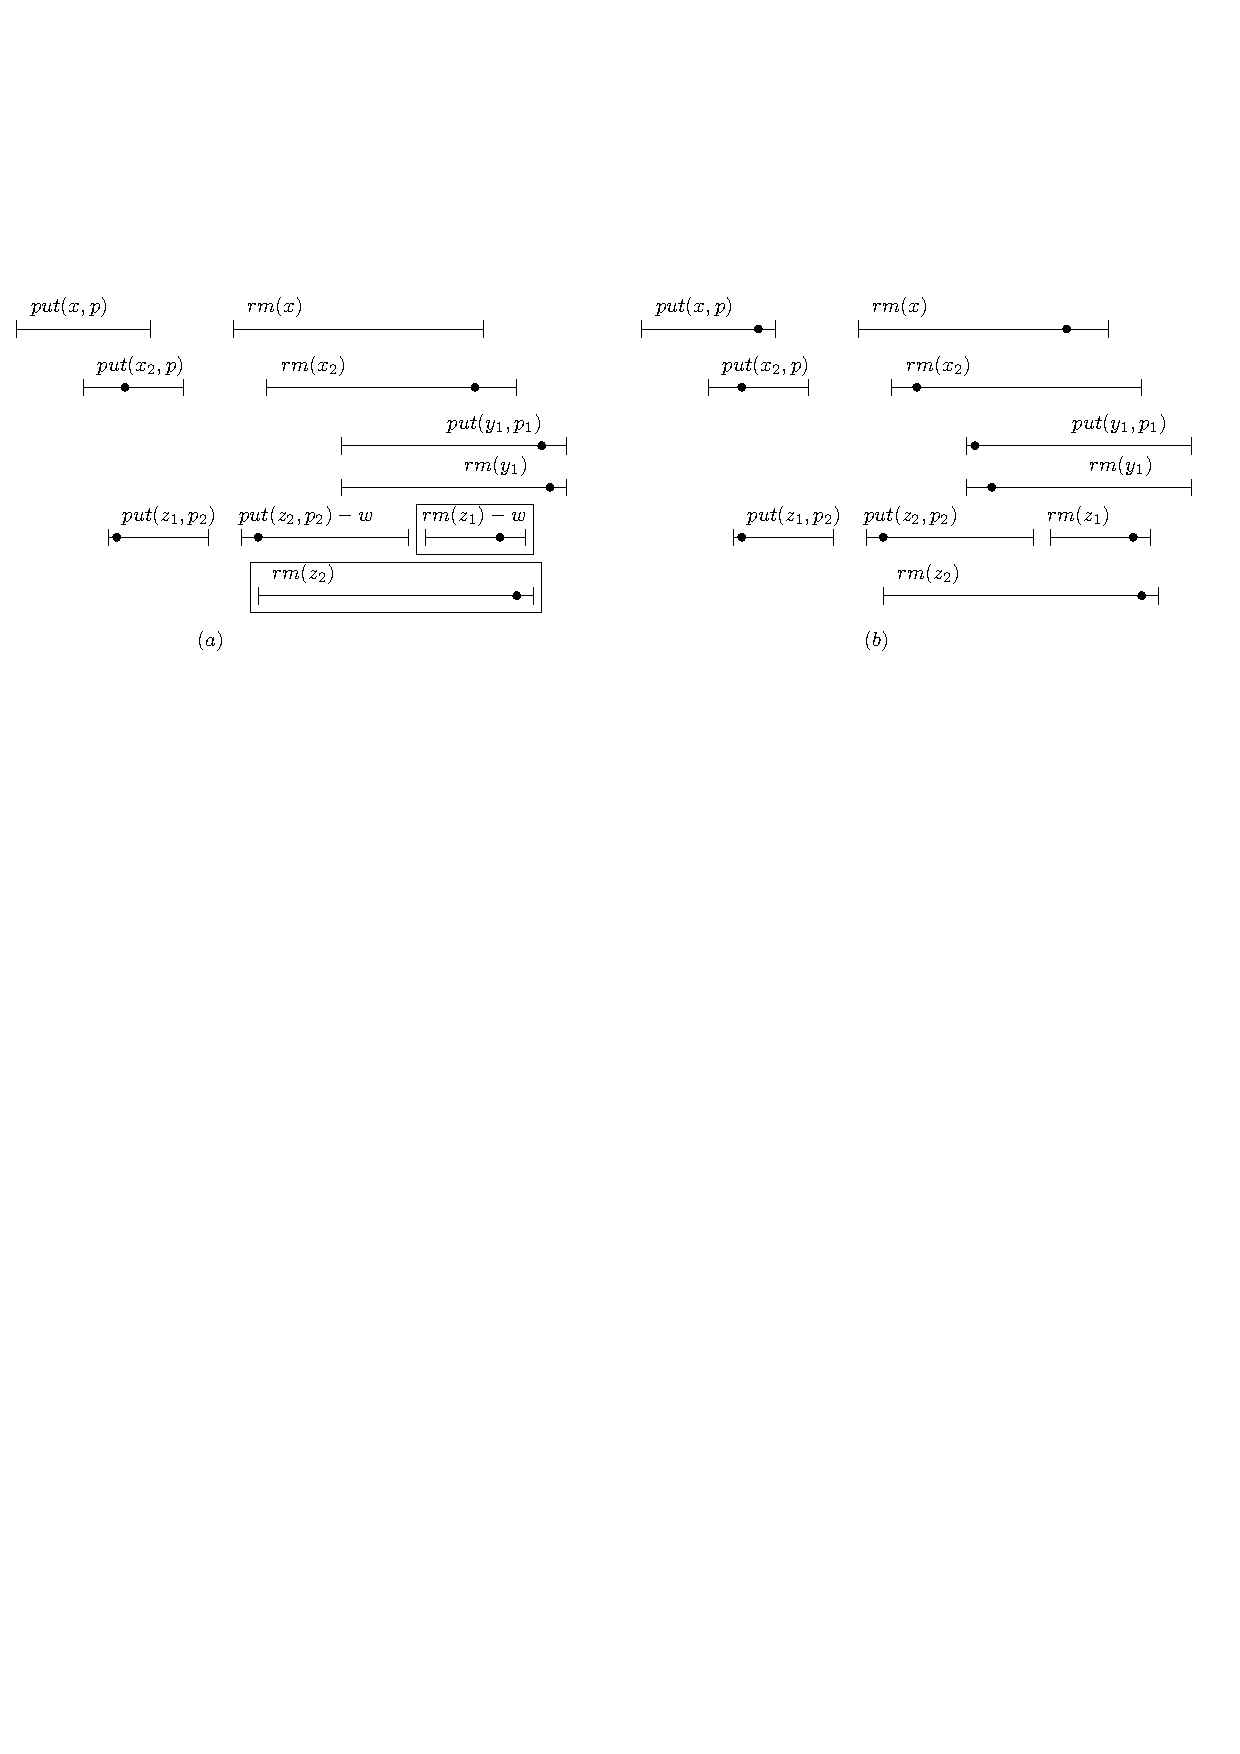
\includegraphics[width=.8\textwidth]{figures/PIC-HIS-EPQ1-TwoHis-2.pdf}
  \caption{A concurrent execution $e$ exemplifying the soundness of $\textit{Check-PQ-Conc}$.}
  \label{fig:concurrent execution for EPQ1}
\end{figure}




Section~\ref{sec:co-regular of extended priority queues} introduces a characterization of concurrent priority queue violations using a set of \emph{non-recursive} automata (whose states consist of a fixed number of registers), whose standard synchronized product is equivalent to $\textit{Check-PQ-Conc}$ (modulo a renaming of values which is possible by data-independence). Since $\seqPQ$ is closed under projection (Lemma~\ref{lem:closure_proj}), the recursion in $\textit{Check-PQ-Conc}$ can be eliminated by checking that each projection of a given execution $e$ passes a non-recursive version of $\textit{Check-PQ-Conc}$ where every recursive call $\text{{\bf return}}\ \textit{Check-PQ-Conc}(\ldots)$ is
replaced by  $\text{{\bf return}}\ \mathsf{true}$. Let $\textit{Check-PQ-Conc-NonRec}$ be the thus obtained procedure.

\begin{lemma}
\label{lemma:EPQ as multi in MRpri for history}
Given a data-differentiated execution $e$, $e \sqsubseteq \seqPQ$ if and only if for each $e' \in \textit{proj}(e)$, $\textit{Check-PQ-Conc-NonRec}(e')$ returns $\mathsf{true}$.
\end{lemma}